\documentclass[11pt]{article}

\usepackage[margin=1in]{geometry}
\usepackage[T1]{fontenc}
\usepackage[utf8]{inputenc}
\usepackage{microtype}
\usepackage{booktabs}
\usepackage{amsmath}
\usepackage{amssymb}
\usepackage{graphicx}
\usepackage{float}
\usepackage{xcolor}
\usepackage{hyperref}
\usepackage[numbers,sort&compress]{natbib}

\emergencystretch=2em

\hypersetup{
  colorlinks=true,
  linkcolor=black,
  citecolor=blue!50!black,
  urlcolor=blue!50!black
}

\title{Compute-Selected Generated-Video Content Pockets Predict Delayed Human Recognition}
\author{
  Jawaun Brown\\
  Independent Research Project\\
  \texttt{jawaun@example.com}
}
\date{Preprint draft, June 2026}

\begin{document}
\maketitle

\begin{abstract}
Brain-predictive and self-supervised video models can rank generated videos, but
proxy scores do not by themselves establish that people remember the selected
clips. We test a narrow prediction from a Stable Video Diffusion replay regime:
two content pockets, orange flowers and hanging clothes, were first stabilized
by TRIBE/BMD replay residuals and exact V-JEPA verifier geometry against hard
negative controls. We then froze a two-session old-vs-lure recognition task and
ran a delayed Prolific study. In the complete Wave 2 sample, 62 participants
submitted 25 forced-choice recognition trials each. After excluding
media-error-flagged trials, primary positive pockets were recognized on 114/123
trials (92.7\%, Wilson 95\% CI [86.7\%, 96.1\%]), compared with 150/186 hard
negative control trials (80.6\%, [74.4\%, 85.7\%]). The participant-level
primary-positive minus hard-control contrast was +11.7 percentage points
(bootstrap 95\% CI [+4.4, +19.4], sign-flip $p=0.00425$). Hanging clothes was
individually robust; orange flowers was high in absolute recognition but weaker
as a standalone contrast. These results support a narrow claim: compute-selected
generated-video content pockets can predict delayed human old-vs-lure
recognition advantage. They do not establish broad human memorability,
measured-fMRI/BMD grounding, prompt-conditioned generation control, or a general
black-box optimization result.
\end{abstract}

\section{Introduction}

Video generators make it increasingly cheap to sample many plausible clips for a
single creative intent. The bottleneck then shifts from generation to selection:
which generated clips are likely to matter to a viewer? Standard video
generation metrics emphasize visual quality, temporal consistency, text-video
alignment, or broad preference \citep{huang2023vbench,liu2023fetv}. Those
metrics are necessary, but they do not directly ask whether viewers will
remember the clip.

Human memorability is partly stable across observers and can be predicted from
visual and semantic representations \citep{isola2011memorability,
cohendet2019videomem,newman2020memento}. Brain-aligned video representations
and neural-response prediction models provide another candidate frame:
generated clips can be scored by predicted cortical response, self-supervised
video embeddings, and related descriptor geometry \citep{lahner2024boldmoments,
tribev2,bardes2025vjepa2}. However, a score in a proxy model is not a human
memory result. A generated-video candidate selected by TRIBE, V-JEPA, CLIP, or
any other model must still clear a behavioral gate before the word
``memorability'' is used strongly.

This preprint isolates one such gate. Earlier compute-side audits in our
image-conditioned Stable Video Diffusion (SVD) replay regime
\citep{blattmann2023stablevideodiffusion} found that replay residuals were
dominated by seed-image/content identity rather than by alpha/guidance recipe
choice. Orange flowers and hanging clothes emerged as the strongest
non-jellyfish positive content pockets. Aerial beach, city street, and storm
beach served as hard negative controls. Descriptor-conditioned replication
showed that the primary orange/hanging pockets transported under fresh
stochastic seeds with positive TRIBE scores and exact V-JEPA support, while the
hard controls stayed negative. Generated-video CLIP did not pass prospectively,
so the validation packet was explicitly V-JEPA-caveated.

The present contribution is intentionally modest:

\begin{enumerate}
  \item We translate a compute-proxy content-pocket finding into a frozen
        two-session delayed recognition-memory task.
  \item We use same-category lures and hard negative controls so the task is not
        merely category familiarity.
  \item We show that the pooled primary content-pocket packet is recognized more
        accurately than hard controls.
  \item We keep the claim narrow: delayed old-vs-lure recognition for this
        generated-video packet, not broad memorability or generator steering.
\end{enumerate}

\section{Related Work}

\paragraph{Visual and video memorability.}
Image memorability work showed that some images are consistently remembered
better than others across observers \citep{isola2011memorability}. Video
memorability extends this to dynamic clips, semantic events, and temporal decay
\citep{cohendet2019videomem,newman2020memento}. The MediaEval video
memorability tasks further separate short-term memorability, long-term
memorability, dataset generalization, and EEG-adjacent prediction subtasks
\citep{sweeney2022mediaeval}. These results motivate behavioral validation, but
they do not remove the need to test generated-video stimuli directly.

\paragraph{Brain-aligned and self-supervised video representations.}
BOLD Moments links short naturalistic videos, fMRI responses, and memorability
metadata \citep{lahner2024boldmoments}. TRIBE v2 is a multimodal
brain-encoding model for predicting cortical responses from vision, audition,
and language \citep{tribev2}. V-JEPA-style self-supervised video models provide
a strong non-brain representation frame for video understanding
\citep{bardes2025vjepa2}. In the current study, TRIBE and V-JEPA are used to
select and verify candidate pockets, not as substitutes for human behavior.

\paragraph{Brain-to-media and response-guided generation.}
Recent fMRI-to-image and fMRI-to-video systems use diffusion models,
CLIP-style conditions, semantic guidance, and temporal reconstruction modules to
reconstruct perceived content from brain activity
\citep{lu2023minddiffuser,chen2023mindvideo,gong2024neuroclips,
sun2024neurocine,yang2026semvideo}. Conversely, response-guided and
saliency-guided generation methods use neural or attention predictors to steer
image synthesis \citep{pierzchlewicz2023energyguided,zhang2025gazefusion,
wang2024sgool}. Our setting is different: we do not decode media from measured
brain activity, and we do not claim a differentiable neural reward for video
generation. We test whether a compute-selected generated-video content pocket
survives delayed human recognition.

\section{Compute-Side Candidate Regime}

\subsection{Artifact regime}

The candidate pool consists of seed images, image-conditioned SVD generations,
fixed recipe neighborhoods, visual-gate statuses, TRIBE/BMD replay scores,
exact V-JEPA video features, CLIP diagnostics, and pocket labels. Prompt text is
metadata-only in the current SVD replay runner, so prompt rewriting is not an
active image-generation intervention in this regime.

\subsection{Primary and control pockets}

The primary positive pockets are orange flowers and hanging clothes. The hard
negative controls are aerial beach, city street, and storm beach. Blue jellyfish
and old car were retained as secondary boundary pockets in the broader research
ledger, but they are not part of the primary human-recognition claim here.

\subsection{Prospective verifier boundary}

Fresh descriptor-conditioned replication generated and scored 90/90 clips with
zero visual failures. Orange flowers and hanging clothes stayed positive under
TRIBE; hard controls stayed negative. Exact V-JEPA transported prospectively,
but generated-video CLIP did not. The human validation packet was therefore
allowed to use orange/hanging as TRIBE/V-JEPA-verified primary pockets, while
not claiming a two-descriptor V-JEPA+CLIP prospective pass.

\section{Human Recognition-Memory Study}

\subsection{Stimuli}

Each participant saw one old target from each analysis arm in Session 1.
Session 2 presented each old target against a newly generated same-category
lure. Sparse forms prevented any participant from seeing multiple old targets
from the same analysis arm. Fillers were included to stabilize the cover task
and reduce the salience of the five analysis arms.

\begin{table}[t]
\centering
\caption{Analysis arms in the delayed old-vs-lure recognition task.}
\begin{tabular}{lll}
\toprule
Arm & Group & Role \\
\midrule
Orange flowers & Primary positive & TRIBE/V-JEPA-verified candidate pocket \\
Hanging clothes & Primary positive & TRIBE/V-JEPA-verified candidate pocket \\
Aerial beach & Hard negative control & Matched negative content pocket \\
City street & Hard negative control & Matched negative content pocket \\
Storm beach & Hard negative control & Matched negative content pocket \\
\bottomrule
\end{tabular}
\end{table}

\subsection{Procedure}

Session 1 was a viewing and cover-task session. Session 2 was a delayed
two-alternative forced-choice recognition task: participants selected which clip
they had seen in Session 1. Participant identifiers were used only for study
matching/payment and were reduced to aggregate counts in committed analysis
artifacts. The endpoint is exact old-vs-lure recognition accuracy, which is
stronger than preference but narrower than free recall, long-term memory, or
measured neural validation.

\subsection{Data integrity}

The Wave 2 Prolific export contained 64 rows: 60 approved, 2 awaiting review,
and 2 timed out. The webhook export contained complete real Session 2 payloads
for all 62 completed submissions and none for the two timed-out submissions.
There were no duplicate real Prolific IDs in complete Session 2 payloads.

The Wave 1 webhook inbox was capped before a paid upgrade, so the full Session 1
JSON payload set is not available. The retained Wave 1 subset contains 24
complete payloads; 21 overlap with complete Wave 2 participants, and all 21
have matching deterministic form assignments. We therefore report the result as
Prolific-confirmed Wave 1 exposure plus complete Session 2 recognition, with
partial Wave 1 JSON retention as a provenance caveat.

\subsection{Analysis}

Primary analyses exclude trials flagged with media errors. We report Wilson
confidence intervals for binomial recognition accuracy, exact binomial tests
against chance, and participant-level paired contrasts between the primary
positive packet and the hard-control pool. Paired uncertainty is estimated with
bootstrap resampling over participants. A sign-flip permutation test evaluates
whether the paired primary-minus-hard contrast differs from zero.

\section{Results}

\subsection{Recognition accuracy}

\begin{figure}[H]
\centering
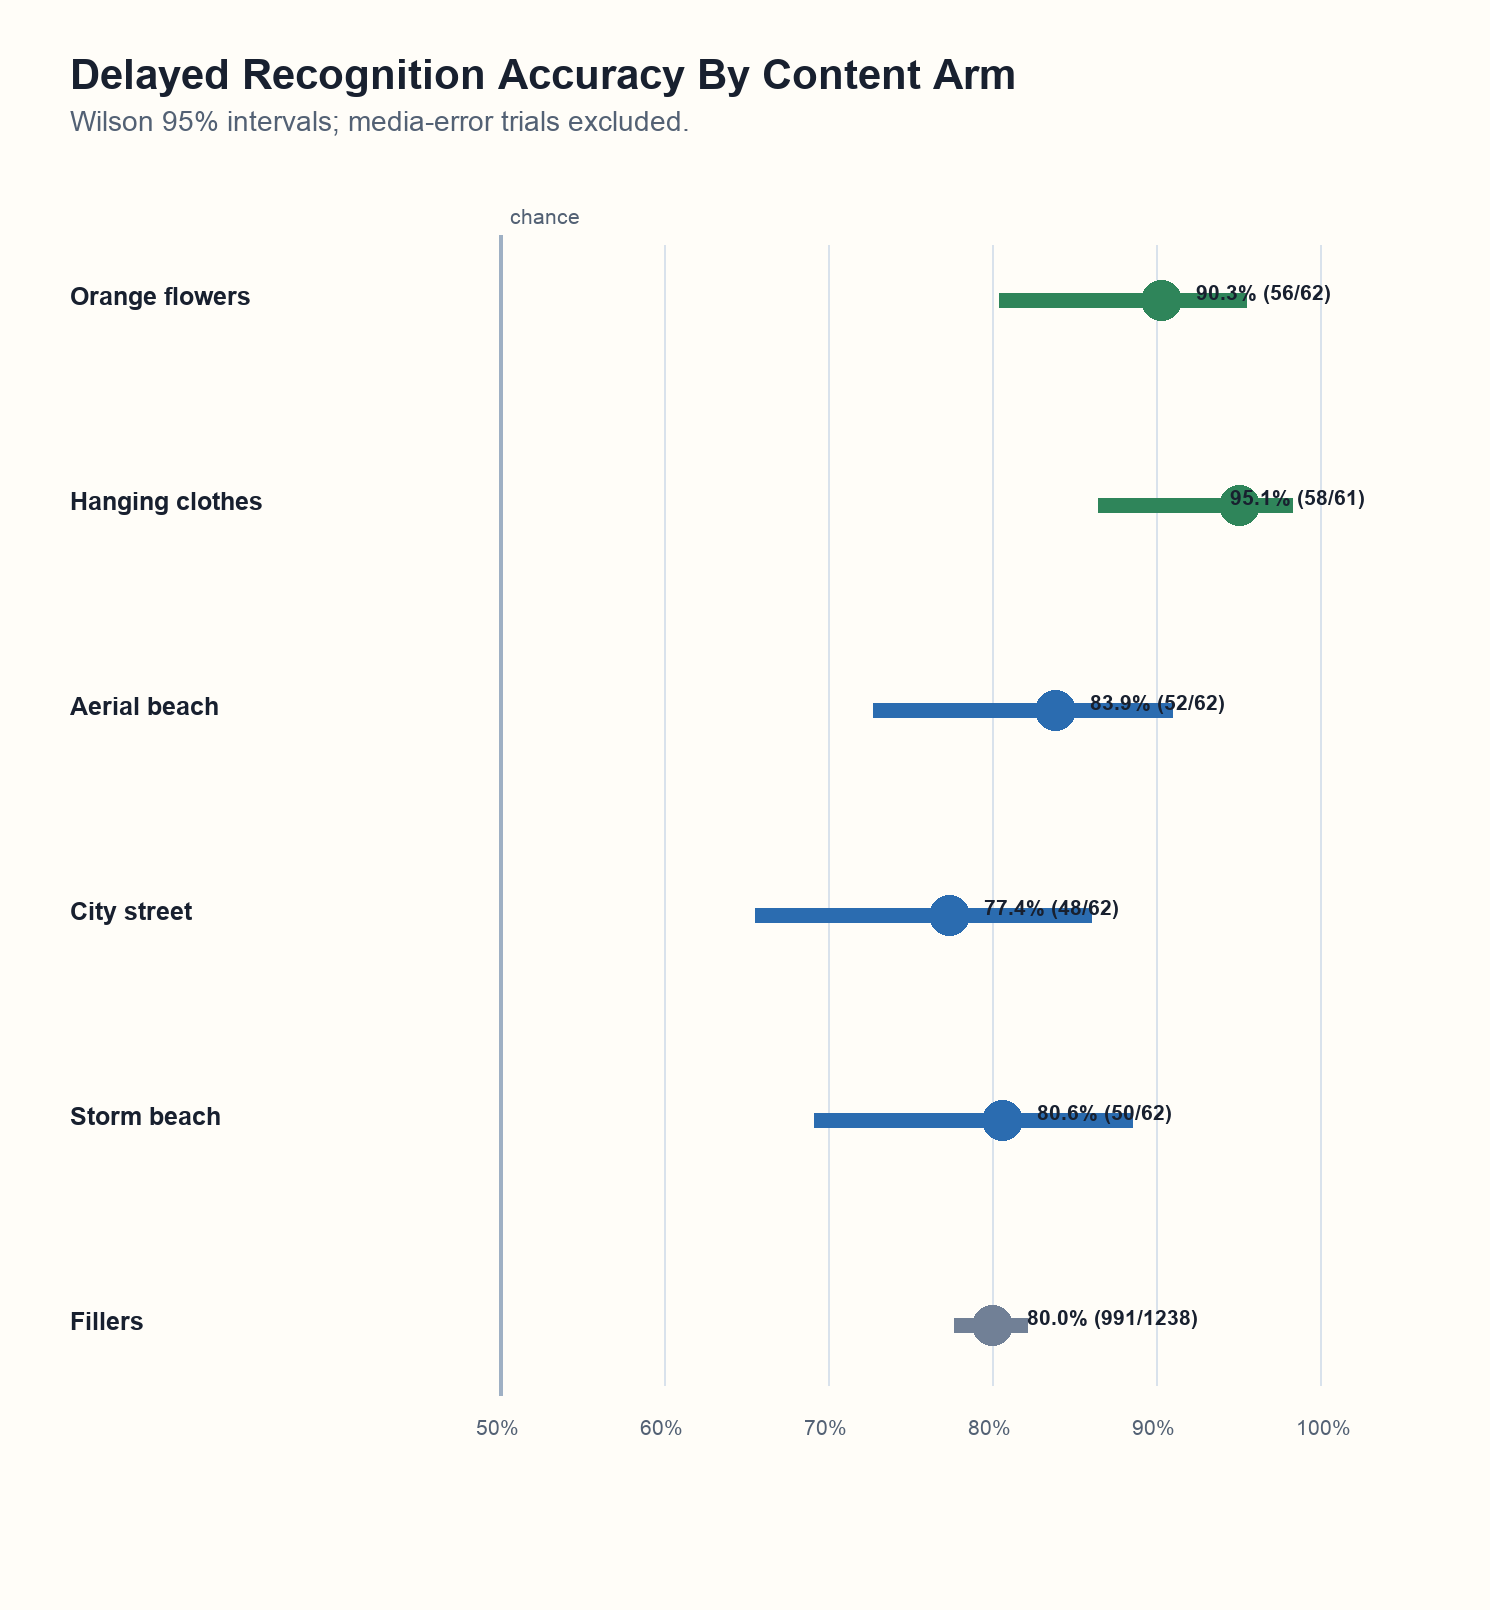
\includegraphics[width=0.95\linewidth]{figures/recognition_accuracy.png}
\caption{Delayed old-vs-lure recognition accuracy by content arm after
excluding media-error-flagged trials. Points show accuracy and horizontal bars
show Wilson 95\% confidence intervals.}
\label{fig:accuracy}
\end{figure}

\begin{table}[t]
\centering
\caption{No-media-error recognition results.}
\begin{tabular}{lrrrr}
\toprule
Group & Correct / $n$ & Accuracy & Wilson 95\% CI & Exact $p$ vs 0.5 \\
\midrule
Primary positives & 114 / 123 & 0.927 & [0.867, 0.961] & $2.68\times10^{-24}$ \\
Hard negative controls & 150 / 186 & 0.806 & [0.744, 0.857] & $9.63\times10^{-18}$ \\
Unrelated fillers & 991 / 1238 & 0.800 & [0.777, 0.822] & $7.69\times10^{-106}$ \\
Orange flowers & 56 / 62 & 0.903 & [0.805, 0.955] & $2.97\times10^{-11}$ \\
Hanging clothes & 58 / 61 & 0.951 & [0.865, 0.983] & $3.29\times10^{-14}$ \\
Aerial beach & 52 / 62 & 0.839 & [0.728, 0.910] & $5.71\times10^{-8}$ \\
City street & 48 / 62 & 0.774 & [0.656, 0.860] & $1.74\times10^{-5}$ \\
Storm beach & 50 / 62 & 0.806 & [0.691, 0.886] & $1.21\times10^{-6}$ \\
\bottomrule
\end{tabular}
\end{table}

The hard negative controls were also recognized above chance. The result is
therefore not that only the positive pockets are memorable. The supported claim
is relative: the primary positive packet was recognized more accurately than
the hard-control pool under the same sparse old-vs-lure task.

\subsection{Primary packet contrast}

\begin{figure}[H]
\centering
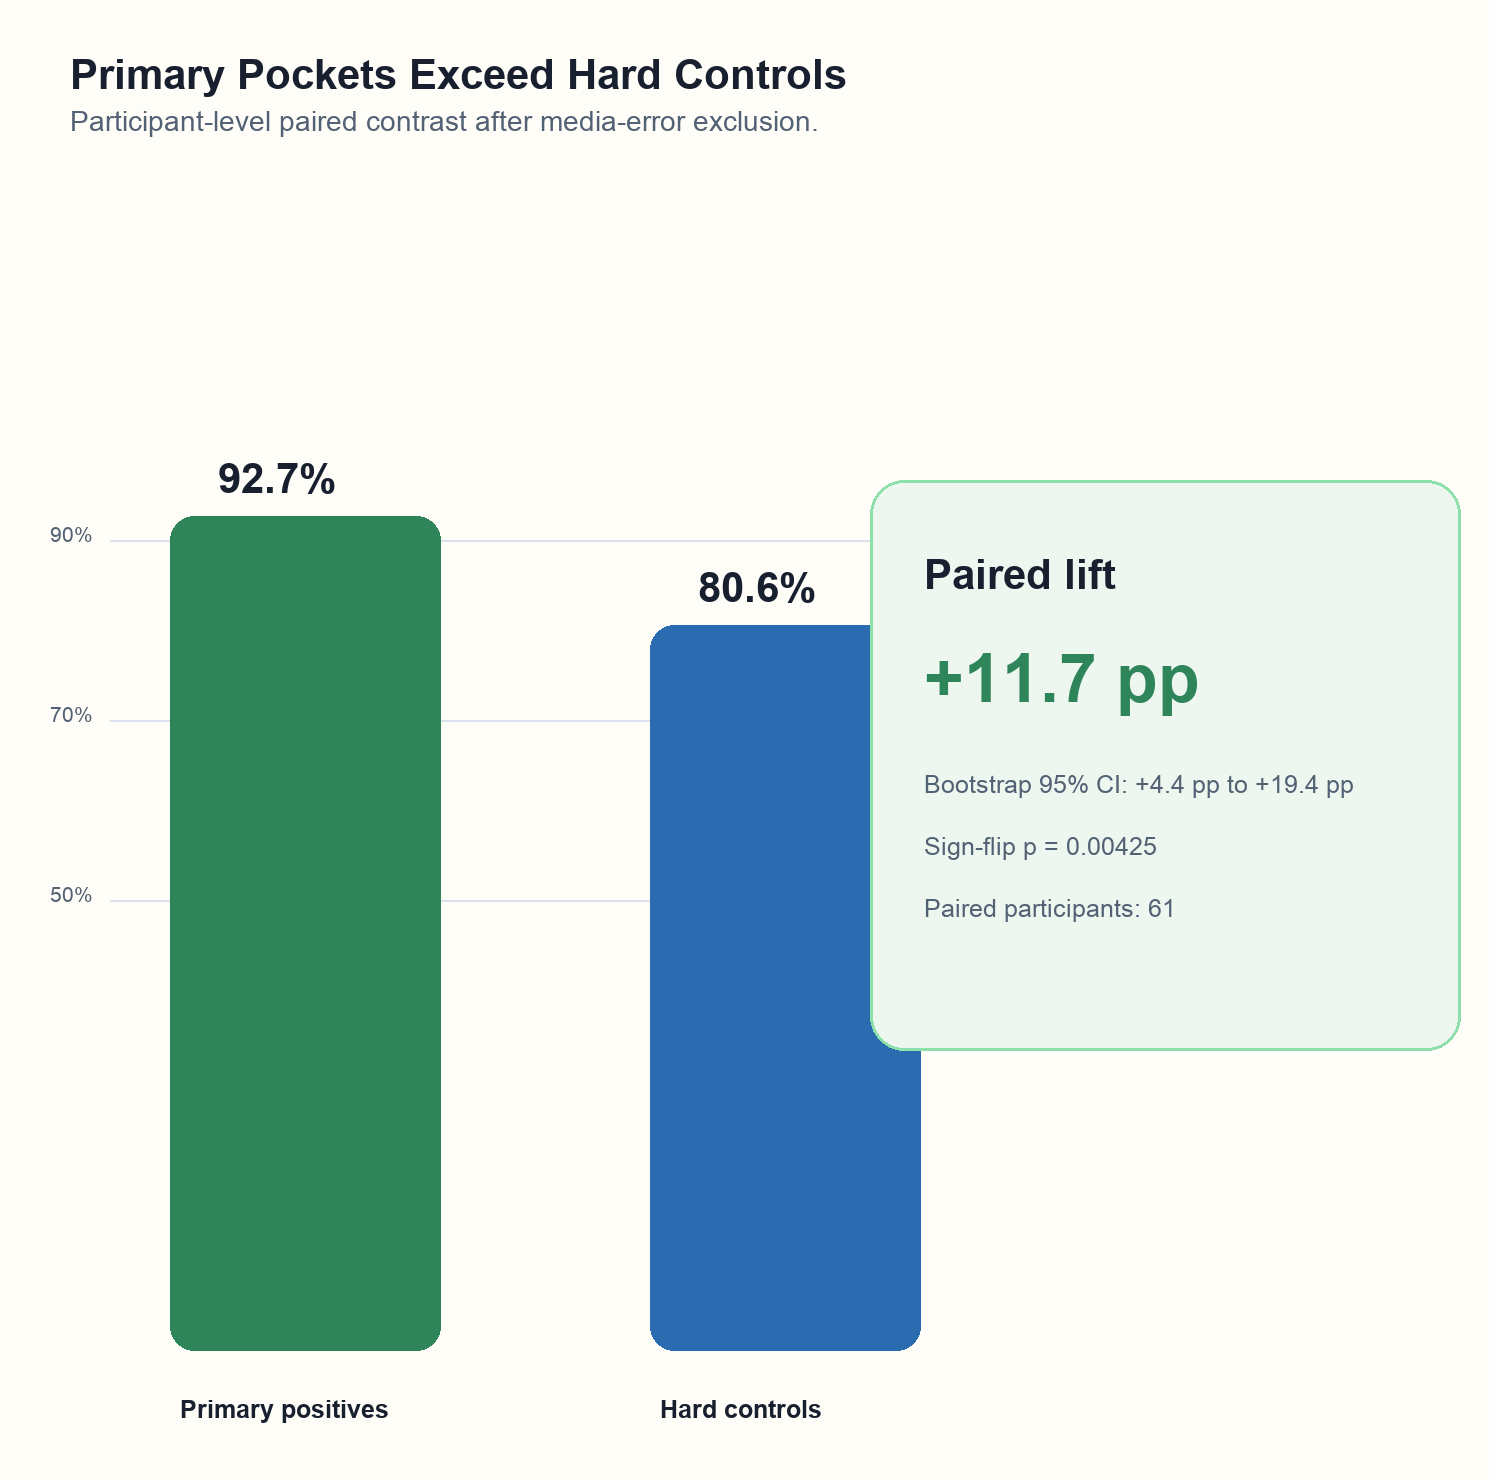
\includegraphics[width=0.86\linewidth]{figures/primary_vs_hard_lift.png}
\caption{Pooled primary-positive packet versus hard controls. The paired
participant-level lift was +11.7 percentage points after excluding
media-error-flagged trials.}
\label{fig:pooled}
\end{figure}

The primary-positive minus hard-control contrast was +11.7 percentage points
(bootstrap 95\% CI [+4.4, +19.4], sign-flip $p=0.00425$) across 61 complete
paired participants after media-error exclusion. The all-trial sensitivity
analysis was qualitatively similar: +12.1 percentage points, bootstrap 95\% CI
[+4.6, +19.9], sign-flip $p=0.00287$, across 62 complete paired participants.

\subsection{Individual pocket contrasts}

\begin{figure}[H]
\centering
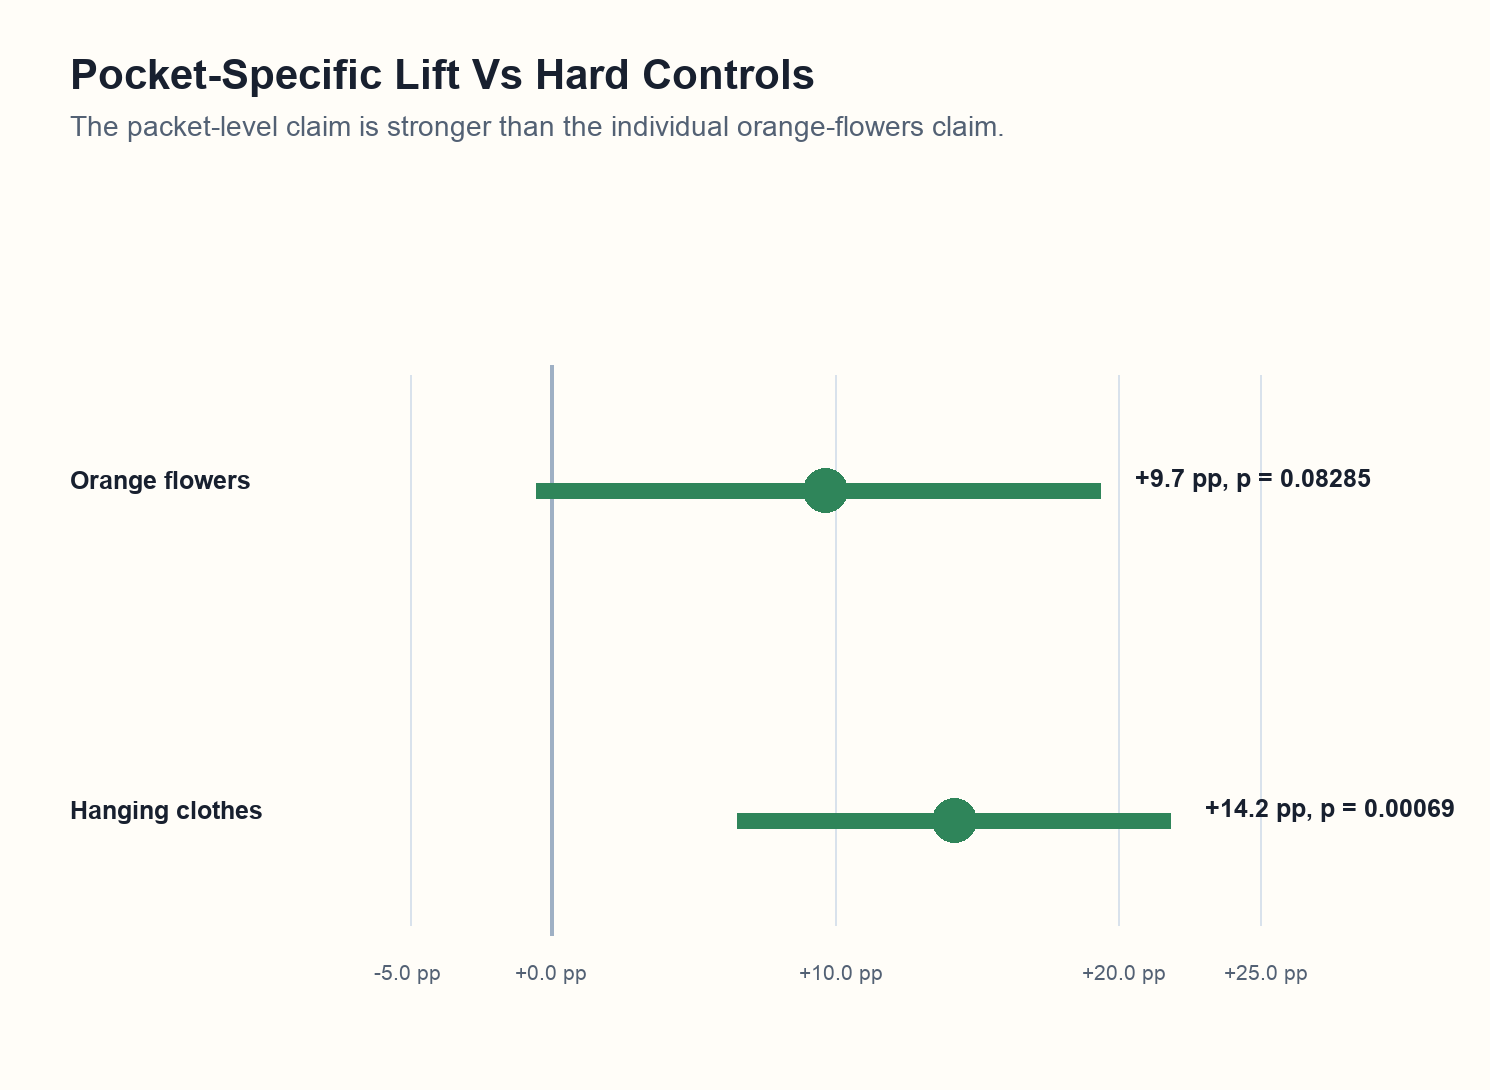
\includegraphics[width=0.9\linewidth]{figures/pocket_specific_lift.png}
\caption{Pocket-specific paired lift versus the hard-control pool. Hanging
clothes clears the individual contrast; orange flowers is high in absolute
recognition but weaker as a standalone hard-control contrast in this wave.}
\label{fig:pockets}
\end{figure}

Hanging clothes exceeded the hard-control pool by +14.2 percentage points
(bootstrap 95\% CI [+6.6, +21.9], sign-flip $p=0.00069$). Orange flowers was
high in absolute recognition but weaker as a standalone contrast: +9.7
percentage points, bootstrap 95\% CI [-0.5, +19.4], sign-flip $p=0.08285$.
The honest claim is therefore the pooled primary packet, with pocket-specific
nuance preserved.

\section{Discussion}

This study upgrades one content-pocket line from compute-proxy evidence to a
narrow human behavioral result. The selection path was prospective at the
claim-relevant level:
\[
\begin{aligned}
&\text{TRIBE/V-JEPA content-pocket candidates}\\
&\rightarrow \text{frozen old-vs-lure stimuli}\\
&\rightarrow \text{delayed human recognition endpoint}.
\end{aligned}
\]

The result does not imply that any arbitrary TRIBE-high generated video is more
memorable to humans. It says that, within this SVD content-pocket packet, the
primary positive pockets selected by the compute regime were later recognized
more accurately than hard controls. Content identity can therefore be a real
memorability-bearing axis in generated-video candidate selection, and future
selector studies should preserve content-pocket controls, same-category lures,
and independent human endpoints.

\section{Limitations}

First, the original full response-analysis plan named a larger minimum usable
sample. This Wave 2 result is strong enough to draft around, but it should not
be presented as a large-sample final confirmation.

Second, the full Wave 1 webhook payload set was not retained because the inbox
was capped before upgrade. Prolific completion and deterministic form
assignment support the exposure record, and the retained Wave 1 subset shows
zero form mismatches, but complete Session 1 JSON provenance is absent.

Third, the task measures exact two-alternative recognition against same-category
lures. It does not measure free recall, long-term memory, attention,
engagement, preference, quality, emotion, virality, or commercial outcomes.

Fourth, the positive pockets are content categories. This result does not prove
that alpha/guidance recipes, black-box optimization, or prompt text caused
memorability improvements. In the current SVD runner, prompt text is metadata
for generation.

Fifth, BMD and measured-fMRI grounding remain separate gates. TRIBE/V-JEPA
helped choose the packet, but this human study is behavioral recognition
evidence, not measured neural validation.

\section{Ethics and Data Availability}

Participants were recruited through Prolific for a minimal-risk online
recognition task involving short generated videos. The committed analysis
artifacts contain aggregate counts and summary statistics only. Raw
Prolific/webhook exports are excluded from the repository because they contain
participant metadata. The reproducible aggregate analysis script and
participant-safe result JSON are included with the source release.

\section{Conclusion}

Compute-selected generated-video content pockets can predict a delayed human
old-vs-lure recognition advantage in this packet. The result is narrow but
important: it gives the content-pocket regime a behavioral foothold while
preserving the distinction between proxy scoring, recognition memory, measured
brain validation, and broad memorability claims.

\appendix

\section{Claim Contract}

Allowed now:
\begin{itemize}
  \item The primary orange/hanging content-pocket packet has delayed
        human old-vs-lure recognition evidence.
  \item Pooled primary positives exceed hard controls in participant-level
        recognition accuracy.
  \item Hanging clothes is individually robust in this wave.
  \item Orange flowers has high absolute recognition and supports the pooled
        primary result, but is weaker as a standalone hard-control contrast.
\end{itemize}

Not allowed:
\begin{itemize}
  \item Human memorability is solved.
  \item BO-generated or TRIBE-selected videos are broadly more memorable to
        humans.
  \item TRIBE/V-JEPA scores are human memory.
  \item Prompt rewriting controls memorability in the current SVD runner.
  \item The result is measured-BMD or fMRI validation.
\end{itemize}

\section{Aggregate Provenance}

The aggregate result is generated by
\path{scripts/summarize_content_pocket_recognition_wave2.py}. Committed
result artifacts are:
\begin{itemize}
  \item \path{content_pocket_recognition_response_analysis_result_20260612.json}
  \item \path{content_pocket_recognition_response_analysis_result_20260612.md}
  \item \path{figures/content_pocket_recognition_accuracy_20260612.svg}
  \item \path{figures/content_pocket_recognition_contrast_20260612.svg}
  \item \path{figures/content_pocket_recognition_arm_contrasts_20260612.svg}
\end{itemize}

\bibliographystyle{unsrtnat}
\bibliography{references}

\end{document}
